\chapter*{Введение}							% Заголовок
\addcontentsline{toc}{chapter}{Введение}	% Добавляем его в оглавление

\newcommand{\actuality}{}
\newcommand{\progress}{}
\newcommand{\aim}{{\textbf\aimTXT}}
\newcommand{\tasks}{\textbf{\tasksTXT}}
\newcommand{\novelty}{\textbf{\noveltyTXT}}
\newcommand{\influence}{\textbf{\influenceTXT}}
\newcommand{\methods}{\textbf{\methodsTXT}}
\newcommand{\defpositions}{\textbf{\defpositionsTXT}}
\newcommand{\reliability}{\textbf{\reliabilityTXT}}
\newcommand{\probation}{\textbf{\probationTXT}}
\newcommand{\contribution}{\textbf{\contributionTXT}}
\newcommand{\publications}{\textbf{\publicationsTXT}}

{\actualityandprogress}. Методы восстановления измерений в задаче компьютерной томографии можно разделить на интегральные и алгебраические. К интегральным относится метод светки и обратной проекции....

{\aim} ~данной работы являются разработка метода реконструкции, позволяющего учесть присутствие в объекте сильнопоглощающих включений, а так же метода численной интерпретации результатов измерений многокомпонентных объектов.

Для достижения поставленной цели были решены следующие {\tasks}:
\begin{enumerate}
  \item построен асимптотически быстрый алгебраический метод реконструкции, основанный на применении быстрого преобразования Хафа.
  \item доказана сходимость построеного алгебраического метода реконструкции, за счет полученного математического выражения градиента быстрого преобразования Хафа.
  \item построен алгоритм реконструкции для объектов, содержащих сильнопоглощающие включения.
  \item построен алгоритм реконструкции, учитывающий покомпонентное ослабление полихроматического спектра.
\end{enumerate}

{\novelty}
\begin{enumerate}
  \item Впервые для реконструкции томографических измерений было применено быстрое преобразование Хафа.
  \item Впервые получено выражение для производной быстрого преобразования Хафа, а так же алгоритм его эффективного вычисления.
  \item Построен алгоритм реконструкции, учитывающий вклад сильно поглощающих включений с помощью оригинальной модели ограничений-неравенств.
  \item Предложена схема обработки данных полихроматического зондирования, при которой восстанавливаются реальные физические концентрации элементов.
\end{enumerate}

{\influence} ~Результаты, полученные в диссертационной работе, используются для обработки данных лабораторных исследований. Построенные алгоритмы лягут в основу программного обеспечения новых моделей промышленных томографов.

Полученное в работе выражение для градиента быстрого преобразования Хафа имеет общетеоретическое значение и уже применяется в области машинного обучения для обратного распространения ошибки в нейронных сетях глубокого обучения через слой БПХ.

{\methods}
Для решения задач реконструкции томографических измерений используются методы теории условной и безусловной оптимизации: градиентные методы оптимизации, квадратичное программирование, регуляризация.
Для ускорения итерации алгебраического метода используются алгоритмы обработки изображений в виде быстрого преобразования Хафа.


{\defpositions}
\begin{enumerate}
  \item Предложен эффективный вычислительный метод решения задачи томографической реконструкции FHT-SIRT, основанный на алгебраическом подходе, который позволяет снизить асимптотическую оценку сложности вычисления итерации с $O(n^3)$ до $O(n^2~\log n)$, что подтвержается численными экспериментами и замерами времени работы программной реализации алгоритма.
  \item Проведено математическое обоснование сходимости предложенного метода.
  \item Предложен метод реконструкции на основе квадратичного программирования, который позволяет уменьшить артефакты на восстановленном изображении, вызванные наличием сильно поглощающих областей в зондируемом объекте.
  \item Предложен алгебраический метод реконструкции для случая полихроматического зондирования, который решает оптимизационную задачу реконструкции относительно линейной комбинации концентраций с ограничениями-неравенствами на их область значений.
\end{enumerate}


{\reliability} полученных результатов обеспечивается модельными экспериментами и численными симуляциями, а так же экспериментами с восстановлением реально измеренных в лабораторных условиях образцов.\ Результаты находятся в соответствии с результатами, полученными другими авторами.


{\probation}
Основные результаты работы докладывались~на: конферециях 
35-я конференция молодых ученых и специалистов «Информационные технологии и системы» (2012, 19 - 25 августа, Петрозаводск, Россия),
11th Biennal Conference on High Resolution X-Ray Diffraction and Imaging (XTOP 2012, St. Petersburg, Russia), 
29th European Conference on Modelling and Simulation (ECMS 2015, Albena, Bulgaria),
Eighth International Conference on Machine Vision (ICMV 2015, Barcelona, Spain),
на общефизическом семинаре ИПТМ РАН (октябрь 2016).

{\contribution} Все результаты диссертации, вынесенные на защиту, получены автором самостоятельно.
Автором самостоятельно реализованы методы восстановления FHT-SIRT из первой главы, барьерных функций из второй, метод взвешанных невязок из третьей, проведены численные экспериметны по обработке реальных и модельных данных.
Постановка задач и обсуждение результатов проводились совместно с научным руководителем.
Генерация модельных данных для экспериментов в полихроматике проводилась аспирантом факультета КН НИУ ВШЭ Ингачевой А.~С. 
Программная имплементация метода мягких ограничений, использованная для сравнения с методом барьерных функций во второй главе, принадлежит Соколову В.~В.
Измерения для экспериментов по восстановлению зуба со свинцовым включением производились на лабоработном источнике ИК РАН в лаборатории рефлектометрии и малоуглового рассеяния.
Многие аспекты исследований в разное время обсуждались с Чукалиной М.~В., Николаевым Д.~П., Бузмаковым А.~В., Ингачевой А.~С., Соколовым В.~В.


\ifthenelse{\equal{\thebibliosel}{0}}{% Встроенная реализация с загрузкой файла через движок bibtex8
    \publications\ Основные результаты по теме диссертации изложены в 11 печатных изданиях, 
    3 из которых изданы в журналах, рекомендованных ВАК, 
    6 "--- в тезисах докладов.%
}{% Реализация пакетом biblatex через движок biber
%Сделана отдельная секция, чтобы не отображались в списке цитированных материалов
  \begin{refsection}%
    \printbibliography[heading=countauthorvak, env=countauthorvak, keyword=biblioauthorvak, section=1]%
    \printbibliography[heading=countauthornotvak, env=countauthornotvak, keyword=biblioauthornotvak, section=1]%
    \printbibliography[heading=countauthorconf, env=countauthorconf, keyword=biblioauthorconf, section=1]%
    \printbibliography[heading=countauthor, env=countauthor, keyword=biblioauthor, section=1]%

    \publications\ Основные результаты по теме диссертации изложены в \arabic{citeauthor} печатных изданиях \nocite{PruBuzNik13, Prun2013Crys, Vestnik2016, Prun2013AutomAndRemCont, buz_jac_2015, chukalina2014xray}, 
    \arabic{citeauthorvak} из которых изданы в журналах, рекомендованных ВАК %\nocite{PruBuzNik13, Prun2013Crys, Vestnik2016}, 
    \arabic{citeauthorconf} "--- в тезисах докладов \nocite{itas2015Prun,itas2015Ingacheva,ecms2015Chukalina, icmv2015Chukalina, embc2013Buzmakov, nikolaevfast}.
  \end{refsection}
} % Характеристика работы по структуре во введении и в автореферате не отличается (ГОСТ Р 7.0.11, пункты 5.3.1 и 9.2.1), потому её загружаем из одного и того же внешнего файла, предварительно задав форму выделения некоторым параметрам

\textbf{Объем и структура работы.} Диссертация состоит из~введения, четырёх глав, заключения и~двух приложений.
%% на случай ошибок оставляю исходный кусок на месте, закомментированным
%Полный объём диссертации составляет  \ref*{TotPages}~страницу с~\totalfigures{}~рисунками и~\totaltables{}~таблицами. Список литературы содержит \total{citenum}~наименований.
%
Полный объём диссертации составляет
\formbytotal{TotPages}{страниц}{у}{ы}{}, включая
\formbytotal{totalcount@figure}{рисун}{ок}{ка}{ков} и
\formbytotal{totalcount@table}{таблиц}{у}{ы}{}.   Список литературы содержит  
\formbytotal{citenum}{наименован}{ие}{ия}{ий}.

\actuality

\section{Задачи, решаемые компьютерной томографией}

Для успешного решения многих прикладных задач необходимой является возможность подробного исследования внутренней структуры объектов без их физического изменения или разрушения.
Речь идет о таких областях применения как медицина, промышленность, биология, геология и др. 
Методы, позволяющие осуществлять такие исследования, назыавются томографическими.

Современное развитие вычислительной техники, повышение ее доступности, появление новых инструментариев обработки информации, развитие алгоритмов и компьютерных наук в целом, делают возможным применение алгоритмов обработки изображений для анализа результатов томографических измерений.
В данной работе рассматриваются методы обработки измерений в методе рентгеновской томографии.
Исследуемый объект зондируется рентгеновским излучением под разными углами, называемыми проекционными.
Данные томографической проекции, т.е. измеренное ослабление рентгеновского излучения, позволяют восстановить внутренние характеристики объекта, а именно пространственное распределение коэффициента ослабления рентгеновского излучения.

Центральную роль в подобных измерениях играет томограф - программно-аппаратный комплекс, в котором совмещены как измерительная часть, так и математическая обработка полученных данных.
Аппаратная часть состоит из источника, держателя образца, оптики и детектора, регистрирующего прошедшее излучение. 
При этом возможны различные конфигурации эксперимента. 
Могут меняться форма зондирующего пучка, его спектр, спектр чувствительности и тип детектора, взаимное расположение детектора, источника и держателя образца.
При этом в приложениях медицины критическую роль играет еще и доза облучения, поглащаемая объектом.

``Сырые данные'', полученные непосредственно после измерений не пригодны для их визуального анализа экспертом.
Для того чтобы получить из измеренных данных, так же называемых синограммой, искомые пространственные распределения характеристик объектов, необходимо произвести дополнительную обработку, называемую методами восстановления компьютерной томографии.
Программную часть томографа составляют алгоритмы восстановления томографических измерений, а так же программы управления механическими частями томографа, детектором и излучателем.
В данной работе рассматриваются проблемы, возникающие именно в алгоритмах восстановления, т.е. в программной части томографа.

\section{Артефакты восстановления}

Метод рентгеновской томографии применятеся для исследования объектов, которые могут различаться по широкому списку параметров: размер, химический состав, динамика изменения внутренней структуры, требования к мощности излучения и др.
Наличие ошибок в восстановленных данных может крайне негативно сказаться на дальнейшем использовании результатов в приложениях.
Например, наличие ложного пика в восстановленной характеристике может быть неверно интерпретировано экспертом-медиком как опухоль.
Из-за наличия шумов модель, напечатанная на 3D-принтере, может оказаться непригодной для дальнейшего прототипирования.
Наконец, отсутствие внутренней особенности на восстановленной картине может коренным образом изменить результаты численного моделирования физических процессов в изучаемом образце.
Таким образом, однин из важнейших задач в разработке алгоритмов восстановления измерений компьютерной томографии --- анализ типов, причин возникновения артефактов и борьба с ними.

В зависимости от области применения, в экспериментальной схеме могут меняться конструкция томографа, спектр зондирующего излучения, точность механических подвижек, форма восстанавливающего луча.
Обычно программное обеспечение, обрабатывающее измеренные данные, не учитывает специфики эксперимента, и решает математическую задачу восстановления без учета физических особенностей полученных входных данных.
Отсутствие учета особенностей измерительной схемы является одной из причин возникновения искажений в полученных изображениях --- так называемых артефактов восстановления.
Для борьбы с артефактами восстановления необходимо вносить в алгоритмы поправки, учитывающие особенности эксперимента, или разрабатывать принципиально новые схемы восстановления данных томографических изерений.
Это может быть эвристическая регуляризация промежуточного результата в процессе итеративного восстановления, модификация постановки оптимизационной задачи, учет физических явлений, проявляющихся только в конкретной экспериментальной схеме и др.


Отсутствие учета специфики проводимых исследований --- не единственная причина возникновения артефактов. 
Неточности, порождающие артефакты восстановления, появляются на каждом этапе формирования картны измерений: аппаратная часть, восстановление и интерпретация полученных результатов.
Ошибки аппаратной части появляются в физической калибровке измерительной аппаратуры, калибровке геометрического расположения элементов в измерительной схеме, а так же при формировании входного сигнала для алгоритмов восстановления. 
К первым можно отнести ошибку в величине суммарной интенсивности излучения источника
В результате восстановленная картина может получиться пересвеченной.
Примером второй причины может служить экспериментальная схема, в которой ось вращения объекта смещена относительно оси ``источник-детектор''.
Наконец, к погрешностям, вносимым аппаратурой, можно отнести шумы матрицы детектора, или наоборот, пересвечивание пикселей детектора.
На этапе алгоритмов восстановления могут быть внесены ошбики, связанные с вычислительной точностью программного обеспечения (overflow\\underflow), сходимостью оптимизационных процедур (локальный минимум, недостижение минимума), слишком агрессивной регуляризацией. 
Последняя возможная причина состоит из ошибок визуализации 3-х мерных восстановленных картин и неправильной их интерпретации.

\subsection{Выводы}
Одна из самых важных задач при восстановлении измерений в задаче компьютерной томографии --- избежать появления артефактов.
Ошибки восстановления могут привести к неправильным дальнейшим применениям измеренных объектов
Ошибки возникают на всех этапах формирования томографии, начиная с физических калибровок в аппаратной части и кончая ошибками в визуализации результата.
При разработке ПО для томографа, нужно иметь в виду как возможные причины ошибок, так и специфику задачи, для которой применяется томограф.

\section{Принцип действия томографа}
\subsection{Устройство томографа}
Опишем основные составные части экспериментальной схемы томографа.
Пример реального экспериментального томографа приведен на рисунке ~\ref{fig:ct_scanner}.

\begin{figure}
\centering
\label{fig:ct_scanner}
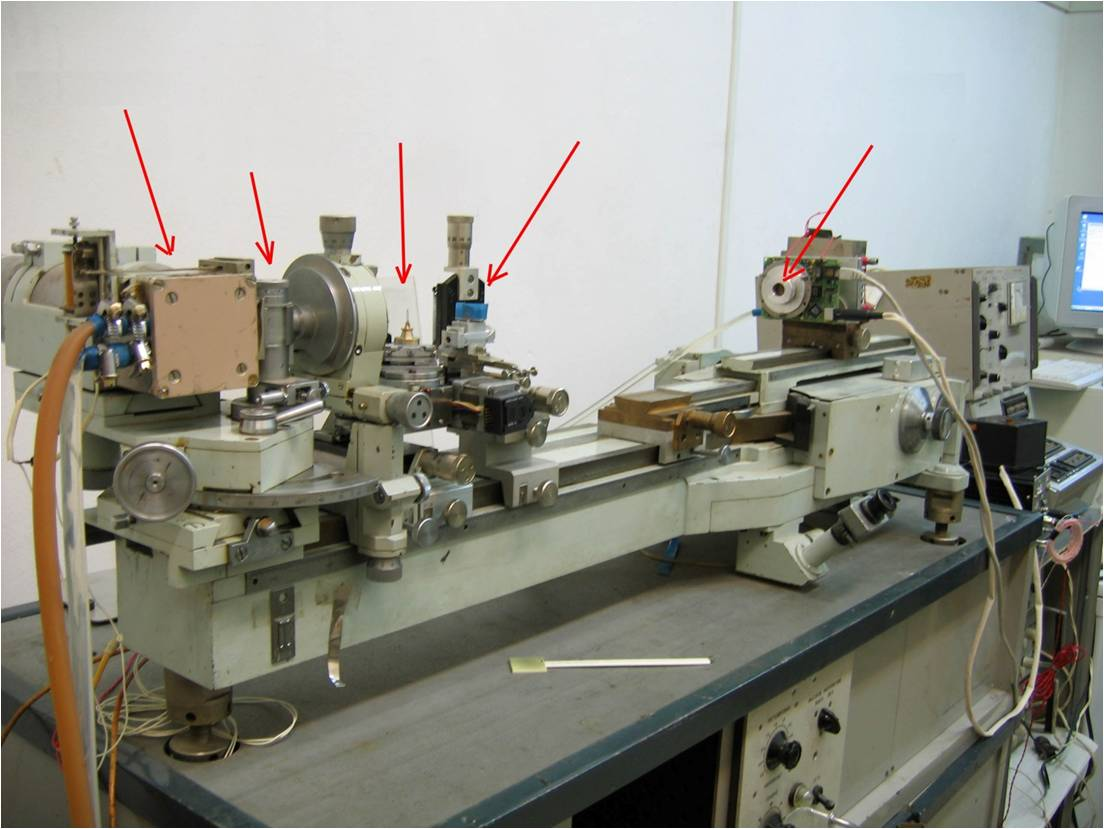
\includegraphics[width=0.7\textwidth]{intro_img/ct_scanner_CIRAS}
\caption{Один из ренгеновских томографов ИК РАН}
\end{figure}

Ренгеновское излучение источника, проходя через предварительные фильтры в виде монохроматора и\\или коллиматора, попадают на объект исследований.
Объект закреплен на вращающейся относительно источника платформе.
Ренгеновское излучение, проходя через объект, поглощается объектом, в результате чего интенсивность излучения ослабляется в соответствии с законом Бугера-Ламберта-Бера:

\begin{equation}
\notag
I = I_0 \exp\left( {-\int \! f(l) \mathrm d l }\right),
\end{equation}

где $l$ -  координата вдоль направления распространения луча, а $f(l)$ - линейный коэффициент ослабления рентгеновского излучения.

Прошедшее через объект излучение затем регистрируется позиционно-чувствительным детектором.
После дискретизации отклика матрицы детектора даные поступают на обработку ПО реконструкции, которое восстанавливает линейный коэффициент ослабления по набору таких измерений объекта под разными углами проекции.
Для того, чтобы понять принцип работы алгоритмов реконструкции, нужно подробнее описать модель формирования измерений.
Проще всего это будет сделать на примере самой простой экспериментальной схемы - экспериментальной схемы с параллельным пучком.

\subsection{Измерения с параллельным пучком}
Несмотря на свою простоту, схема измерений 2D сечения объекта параллельным пучком рентгеновского излучения является ``ядром'' всех алгоритмов восстановления КТ и имеет много применений на практике.
\todo{правильно ли следующее утверждение?}
Параллельный пучок рентгеновского излучения возникает на синхротроне, в лабораторных условиях при использовании монохраматоров, в результате пересчета измерений в веерной 2D геометрии, которая, в свою очередь, возникает в центральном сечении конуского пучка.
Параллельным пучком может обладать только моохроматическое излучение, чем шире спектр тем сильнее расхождение с моделью параллельного пучка.

\begin{figure}[h!]
  \centering
  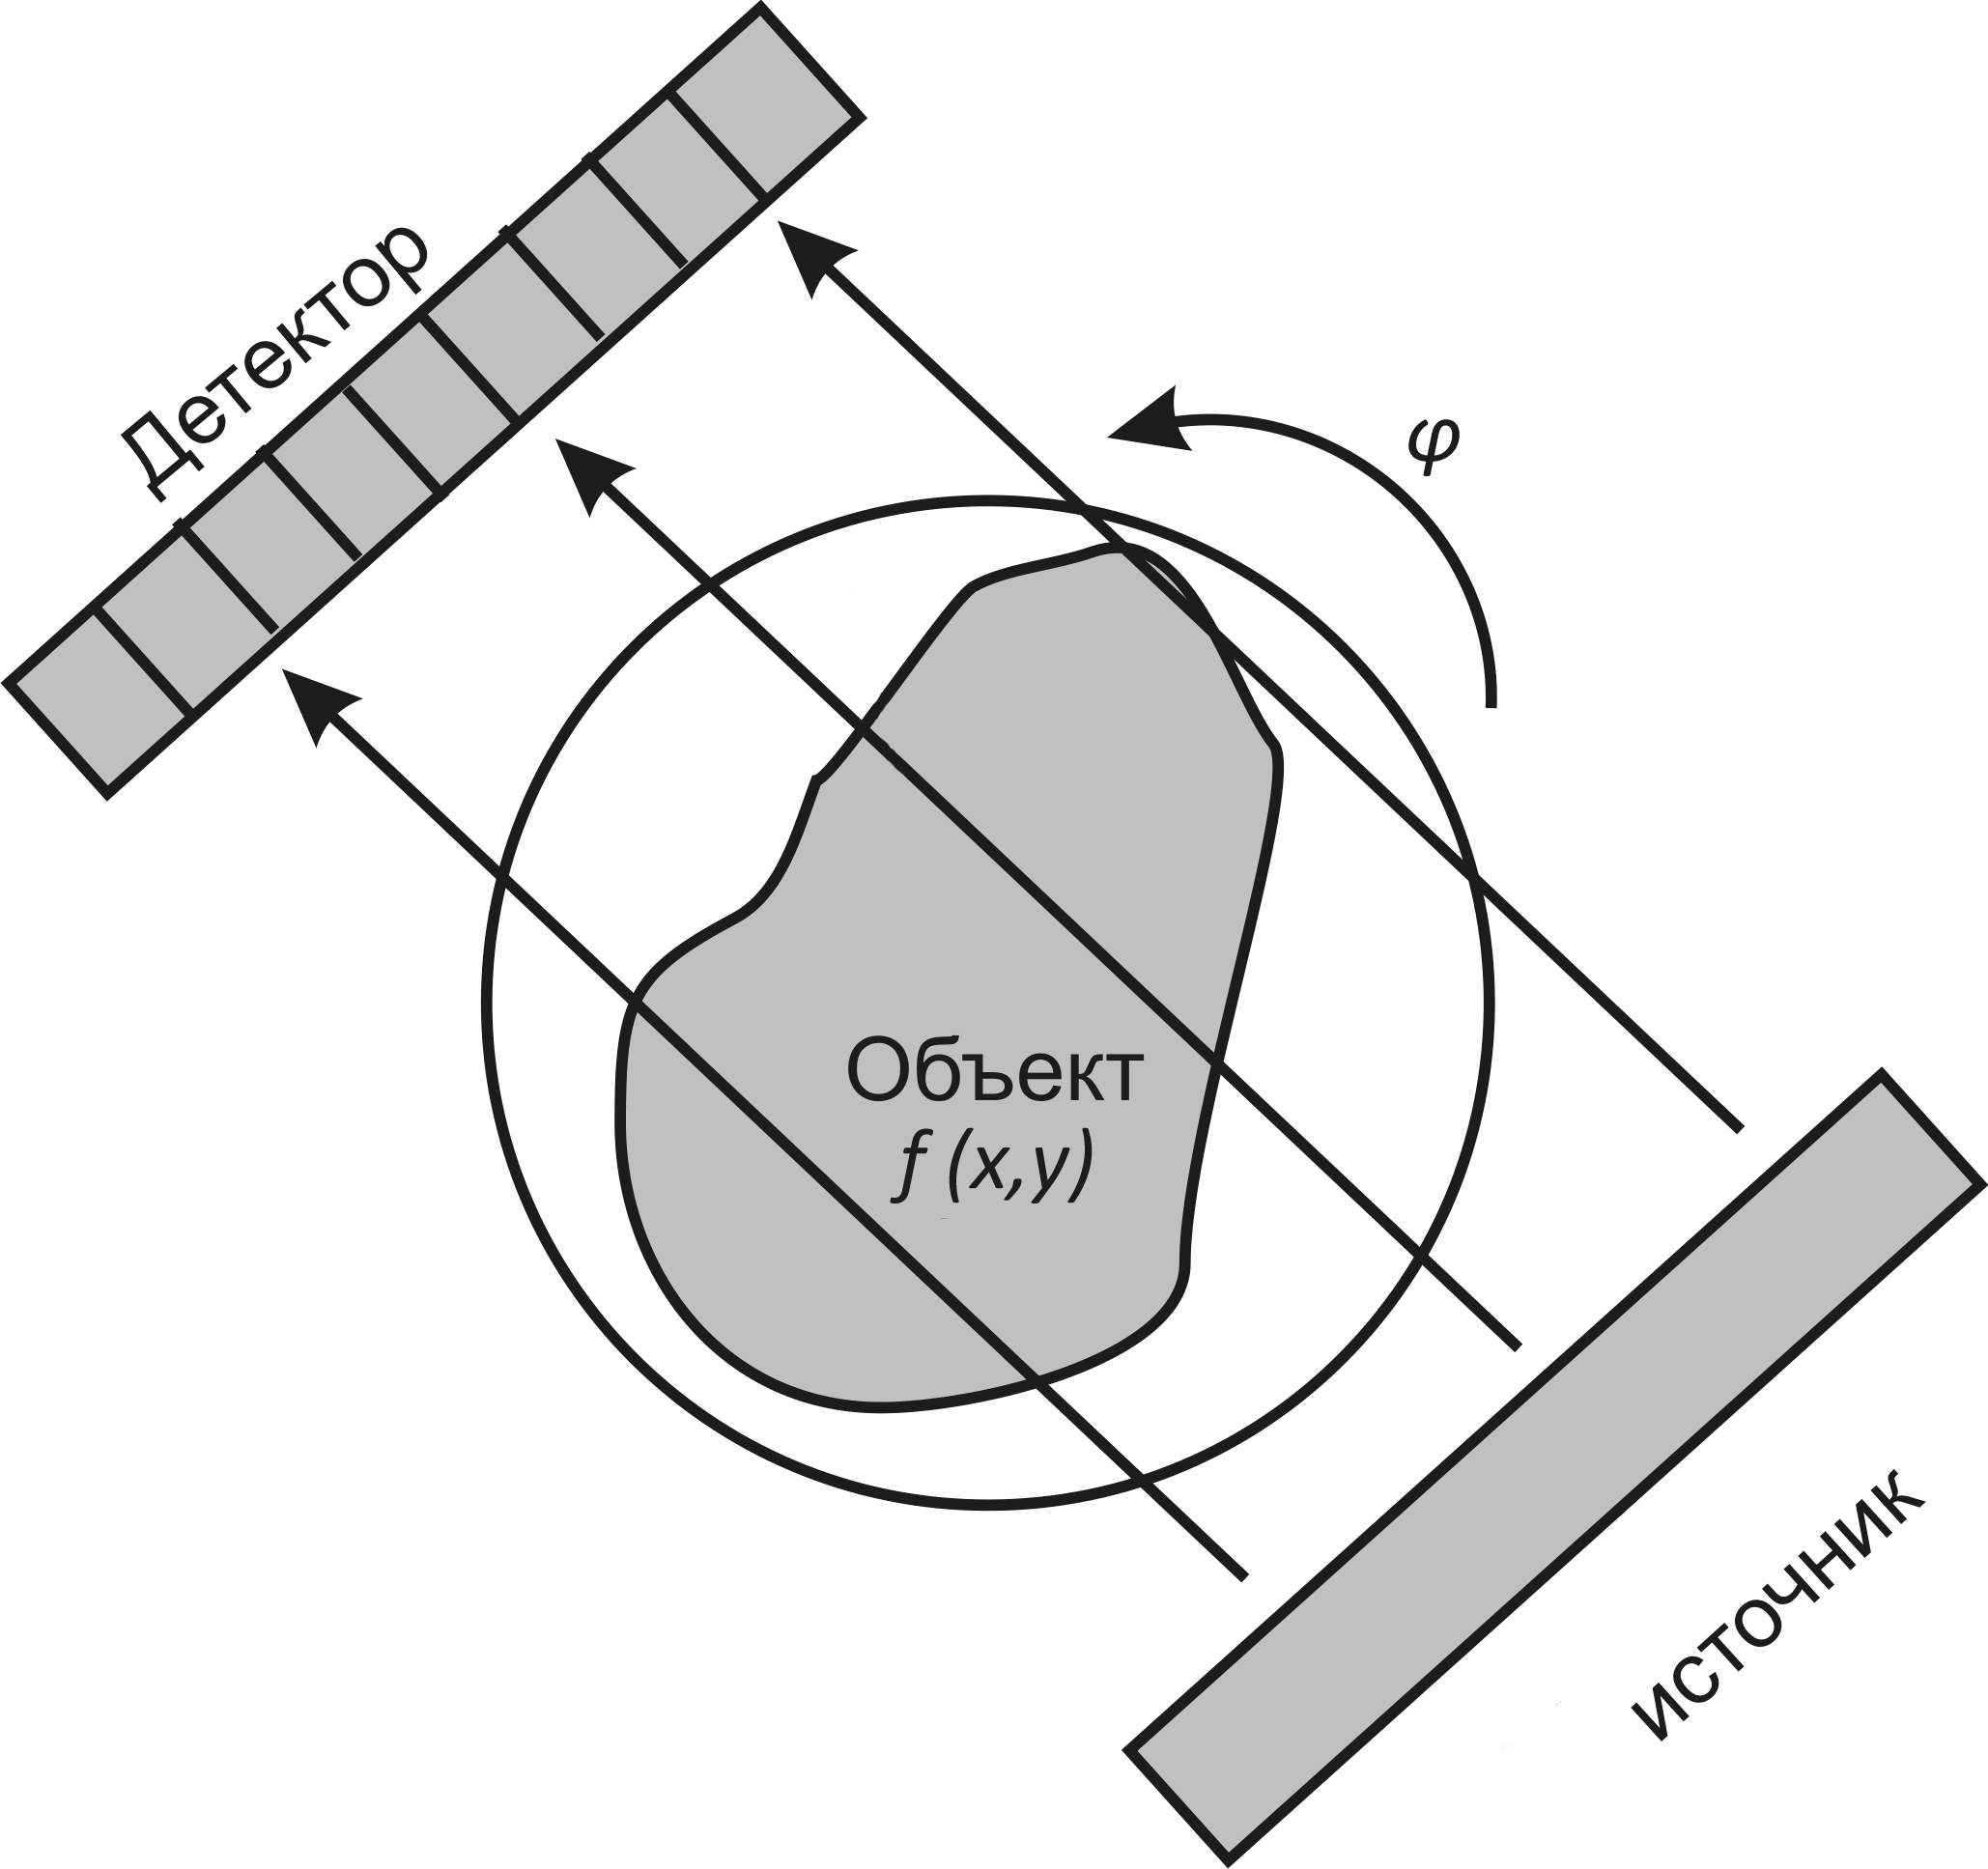
\includegraphics[width=0.5\textwidth]{part1_img/experiment}
  \caption{Схема измерений с параллельным пучком (2D)}
  \label{fig:experiment}
\end{figure}

Схема измерений изображена на рис. ~\ref{fig:experiment}.
Единичного измерения характеризуется двумя параметрами: углом поворота объекта и позицией ячейки детектора, к которой данное измерение относится.
Бесконечно тонкий рентгеновский луч, проходящий под углом $\varphi$  через объект на расстоянии $\xi$  от начала координат, описывается выражением
\begin{equation}\notag
  x\cos\varphi + y\sin\varphi = \xi.
\end{equation}
Тогда регистрируемый в пикселе детектора $\xi$ сигнал имеет интенсивность:
\begin{equation}\notag
  I(\varphi, \xi) = I_0 \exp\left( {-\iint \! \mathrm d x \mathrm d y f(x,y)\delta(x\cos\varphi + y\sin\varphi - \xi)}\right).
\end{equation}
Прологарифмировав обе стороны данного выражения, обозначаем измеренные данные как
\begin{equation}\notag
  p(\varphi, \xi) = \ln \left (\frac{I_0}{I(\varphi, \xi)} \right),
\end{equation}
получим преобразование Радона функции $f(x,y)$:
\begin{equation}\notag
  p(\varphi, \xi)= \iint \! \mathrm d x \mathrm d y f(x,y)\delta(x\cos\varphi + y\sin\varphi - \xi).
\end{equation}
Суть задачи реконструкции в томографии --- восстановление двумерной функции сечения объекта ($f(x,\ y)$) по набору ее линейных интегралов вдоль направлений, соответствующих проекционным углам, по набору проекций ($I(\varphi, \xi)$), или обращение преобразования Радона.

\section{Методы восстановления}
Существует два основных подхода к восстановлению измерений компьютерной томографии.
Первая группа методов ---  интегральные --- подходит к решению задачи обращения преобразования Радона аналитически.
\todo{ базовы формулы про фурье, описание FBP. затем описание принципиальног подхода алгебраического метода, метод карцмарца. После этого про регуляризацию и проч. Про время работы и дальше по плану.}


\todo{дальше как такового введения нет, идут планы и введения из статей, как наработки для копирования текста.}

1. + что такое томография - позволяет без разрушения восстановить внутреннюю структуру в ppt посмотри о видах томографии	

2. + что такое томограф - это аппаратно-программный комплекс, ты будешь в диссере рассматривать проблемы, возникающие в программной части

3. + из Лешиных тезисов - разные объекты требуют разного при реконструкции - отсюда разное качество реконструкции при использовании разных методов реконструкции
  
4. + но не только методы формируют ошибки результатов восстановления - анализ других источников

5. + описываем самое простое измерение - параллельная схема, монохроматический пучок - здесь первое короткое описание модели формирования сигнала в измерительной схеме

6. приходим к выводу, что алгебраические имеют преимущества над интегральными, поскольку можно учесть и влияние аппаратуры и работать при наличии большого шума
но алгебраические медленные - поэтому надо развивать быстрые реализации, хаф

7. усложним задачу. есть сильнопоглощающие включения - часть ко введению из ecms 2015, icmv 2015 подвести к выводу, что надо создавать и в этом простом для измерения случае (параллельный пучок и монохроматика) принципиально новые методы

8. еще усложним задачу - монохроматику заменим полихроматикой и обретем радости с beam-hardening 2 пути решать - честно или постобработкой измеренных проекций или самой восстановленной картинки.

все это дело объединяем еще раз коротко и выводим актуальность работы.

% \section{Обзор литературы}
\begin{comment}

\todo{введение - обзор из статьи аит2013 и бакалаврского диплома}

Компьютерная томография --- это инструмент, широко применяемый сегодня в различных областях жизни, таких как неразрушающий контроль в промышленности, диагностика и лечение  в медицине и др. Целью применения метода компьютерной томографии является реконструкция пространственного распределения характеристик объекта без его физического разрушения. Однако сырые данные, регистрируемые в ходе измерения высокотехнологичными томографическими системами, сами по себе не являются достаточными для описания объекта исследования, а требуют привлечения дополнительного математического аппарата (методов реконструкции изображений, методов визуализации восстановленных изображений и др.). 

Задача восстановления изображения объекта по набору зарегистрированных томографических проекций известна как задача обращения преобразования Радона при условии конечного числа направлений. Методы ее решения, интегральные \cite{herman2013mathematical} и алгебраические \cite{algebraic_methods}, постоянно совершенствуются. Предлагаются новые версии алгоритмов, основанных на алгебраическом подходе, способных работать с сильно зашумлёнными проекциями. Такое условие сформировано необходимостью сокращать время регистрации проекций. Для некоторых применений уменьшение времени регистрации связано с требованием сокращения дозы облучения, для других --- обусловлено высокой динамикой поведения исследуемого объекта. Также следует отметить, что алгебраические методы реконструкции незаменимы, когда речь идет об экспериментах с малым числом проекционных углов и измерениях в ограниченном телесном угле. Только алгебраические методы применимы для решения задач трансмиссионно-эмиссионной томографии, если ослаблением зондирующего и вторичного излучений пренебречь нельзя.

Хотя концептуально алгебраические методы проще интегральных и лучше справляются с наличием высокого уровня шума в проекциях, они проигрывают последним по времени реконструкции. Численные реализации новых быстрых алгоритмов и применение распараллеливания на базе графических процессоров делает алгебраический подход конкурентноспособным с сохранением всех преимуществ его поведения в среде с высоким уровнем шума.

\todo{тут идет копипаст из статьи Соколова. надо перевести и переформулировать.}

Appearance of metal streak artifacts in reconstructed CT images is a known problem \cite{barrett2004artifacts, boas2012ct, nasirudin2015reduction,
park2015computed}. Such artifacts are caused by multiple reasons, including beam hardening, scatter, Poisson noise, motion, and edge effects \cite{boas2012ct}. A variety of tricks are used to avoid these artifacts: hardware tricks including automatic control of the X-ray tube voltage and current modulations, software preprocessing of the projection data before reconstruction - sinograms are filtered using adaptive methods of filtering. For example an adaptive expansion of the detector element size in regions of photon starvation are used \cite{boas2012ct}. One more group of methods carries out measurements using a multi-energy scan \cite{bamberg2011metal}. Also there are methods in which
the core of the reconstruction method takes into account the
mathematical model of a sinogram formation. The statistical reconstruction techniques are used to deal with the metal artifact reduction problem \cite{jmuller2006, buzug2008computed}. Contrary to filtered back-projection group of methods, in those techniques, the influence of each single beam on the image reconstruction can be weighted separately. The maximum likelihood
(MLEM) algorithm \cite{buzug2008computed} and modified MLEM algorithm called $\lambda$-MLEM \cite{oehler2007statistical} improve image quality comparing to pure interpolation or missing data concept \cite{amirkhanov2012evaluation}.

\end{comment}